% !TEX program = lualatex
% Generated by new_homework.sh — Math 104 Homework 2
\documentclass[11pt]{article}

\usepackage{fontspec}
\usepackage{microtype}
\usepackage{mathtools,amssymb,amsfonts,amsthm,bm}
\usepackage{enumitem}
\usepackage{booktabs,array,xcolor}
\usepackage{geometry,fancyhdr,setspace}
\usepackage{pdfpages}
\usepackage[hidelinks]{hyperref}
\usepackage[nameinlink,noabbrev]{cleveref}

% ---------- Page and paragraph rhythm (matches lecture/solutions templates) ----------
\geometry{margin=1in,headheight=15pt}
\setstretch{1.12}
\setlength{\parindent}{0pt}
\setlength{\parskip}{0.55em plus 0.12em minus 0.08em}
\setlength{\abovedisplayskip}{0.8em plus 0.2em minus 0.1em}
\setlength{\belowdisplayskip}{0.8em plus 0.2em minus 0.1em}
\allowdisplaybreaks[3]
\setlist{leftmargin=*,topsep=0.35em,itemsep=0.15em,parsep=0pt}

% ---------- Metadata ----------
\newcommand{\studentname}{Keshav Ramamurthy}
\newcommand{\coursename}{Math 104}
\newcommand{\courselongname}{Real Analysis}
\newcommand{\assignment}{Homework 2}
\newcommand{\term}{Fall 2026}

% ---------- Core notation (same as ~/.config/nvim/textemplate.tex) ----------
\newcommand{\N}{\mathbb{N}}
\newcommand{\Z}{\mathbb{Z}}
\newcommand{\Q}{\mathbb{Q}}
\newcommand{\R}{\mathbb{R}}
\newcommand{\C}{\mathbb{C}}
\newcommand{\F}{\mathbb{F}}
\newcommand{\K}{\mathbb{K}}
\newcommand{\E}{\mathbb{E}}
\newcommand{\Prob}{\mathbb{P}}
\newcommand{\1}{\mathbf{1}}
\newcommand{\eps}{\varepsilon}
\newcommand{\dd}{\,\mathrm{d}}
\newcommand{\abs}[1]{\left\lvert#1\right\rvert}
\newcommand{\norm}[1]{\left\lVert#1\right\rVert}
\newcommand{\ip}[2]{\left\langle#1,#2\right\rangle}
\newcommand{\set}[1]{\left\{#1\right\}}
\newcommand{\ceil}[1]{\left\lceil#1\right\rceil}
\newcommand{\floor}[1]{\left\lfloor#1\right\rfloor}
\newcommand{\given}{\,\middle\vert\,}
\newcommand{\indep}{\perp\!\!\!\perp}
\newcommand{\wh}[1]{\widehat{#1}}
\newcommand{\deriv}[2]{\frac{\mathrm{d}#1}{\mathrm{d}#2}}
\newcommand{\pderiv}[2]{\frac{\partial#1}{\partial#2}}
\newcommand{\lto}{\longrightarrow}
\newcommand{\st}{\text{ such that }}
\DeclareMathOperator{\Aut}{Aut}
\DeclareMathOperator{\End}{End}
\DeclareMathOperator{\Gal}{Gal}
\DeclareMathOperator{\Hom}{Hom}
\DeclareMathOperator{\Ker}{ker}
\DeclareMathOperator{\im}{im}
\DeclareMathOperator{\rank}{rank}
\DeclareMathOperator{\nullity}{nullity}
\DeclareMathOperator{\Span}{span}
\DeclareMathOperator{\tr}{tr}
\DeclareMathOperator{\diag}{diag}
\DeclareMathOperator{\spec}{spec}
\DeclareMathOperator{\ord}{ord}
\DeclareMathOperator{\supp}{supp}
\DeclareMathOperator{\diam}{diam}
\DeclareMathOperator{\Var}{Var}
\DeclareMathOperator{\Cov}{Cov}
\DeclareMathOperator*{\argmin}{arg\,min}
\DeclareMathOperator*{\argmax}{arg\,max}

% ---------- Statement environments ----------
\newtheorem{problem}{Problem}
\newtheorem{theorem}{Theorem}
\newtheorem{lemma}{Lemma}
\newtheorem{proposition}{Proposition}
\newtheorem{corollary}{Corollary}
\theoremstyle{definition}
\newtheorem{definition}{Definition}
\newtheorem{example}{Example}
\newtheorem{remark}{Remark}

% ---------- Solution machinery (matches solutions.tex / textemplate.tex) ----------
\newenvironment{solution}{\begin{proof}[Solution]}{\end{proof}}
\newenvironment{answer}{\begin{proof}[Answer]}{\end{proof}}
\renewcommand{\qedsymbol}{$\square$}
\newcommand{\exercise}[1]{%
  \par\goodbreak\medskip\noindent\textbf{Exercise #1}\par\nopagebreak\smallskip\nopagebreak}
\newcommand{\exref}[1]{\textsf{\textbf{Exercise~#1}}}
\newenvironment{claim}{\par\smallskip\noindent\textbf{Claim.}\ }{\par\smallskip}
\newenvironment{idea}{\par\smallskip\noindent\textit{Idea.}\ }{\par\smallskip}
\newenvironment{proofsketch}{\par\smallskip\noindent\textbf{Proof sketch.}\ }{\par\smallskip}

% ---------- Header ----------
\pagestyle{fancy}
\fancyhf{}
\fancyhead[L]{\coursename}
\fancyhead[C]{\assignment\ — my solutions}
\fancyhead[R]{\studentname}
\fancyfoot[C]{\thepage}

\begin{document}

% ---------- Title ----------
\begin{center}
  {\Large\sffamily\bfseries \coursename\ -- \courselongname}\par\vspace{3pt}
  {\sffamily \assignment\ — my solutions}\par\vspace{3pt}
  {\small\sffamily \term\quad\textbullet\quad \studentname}
\end{center}
\medskip
\hrule
\bigskip

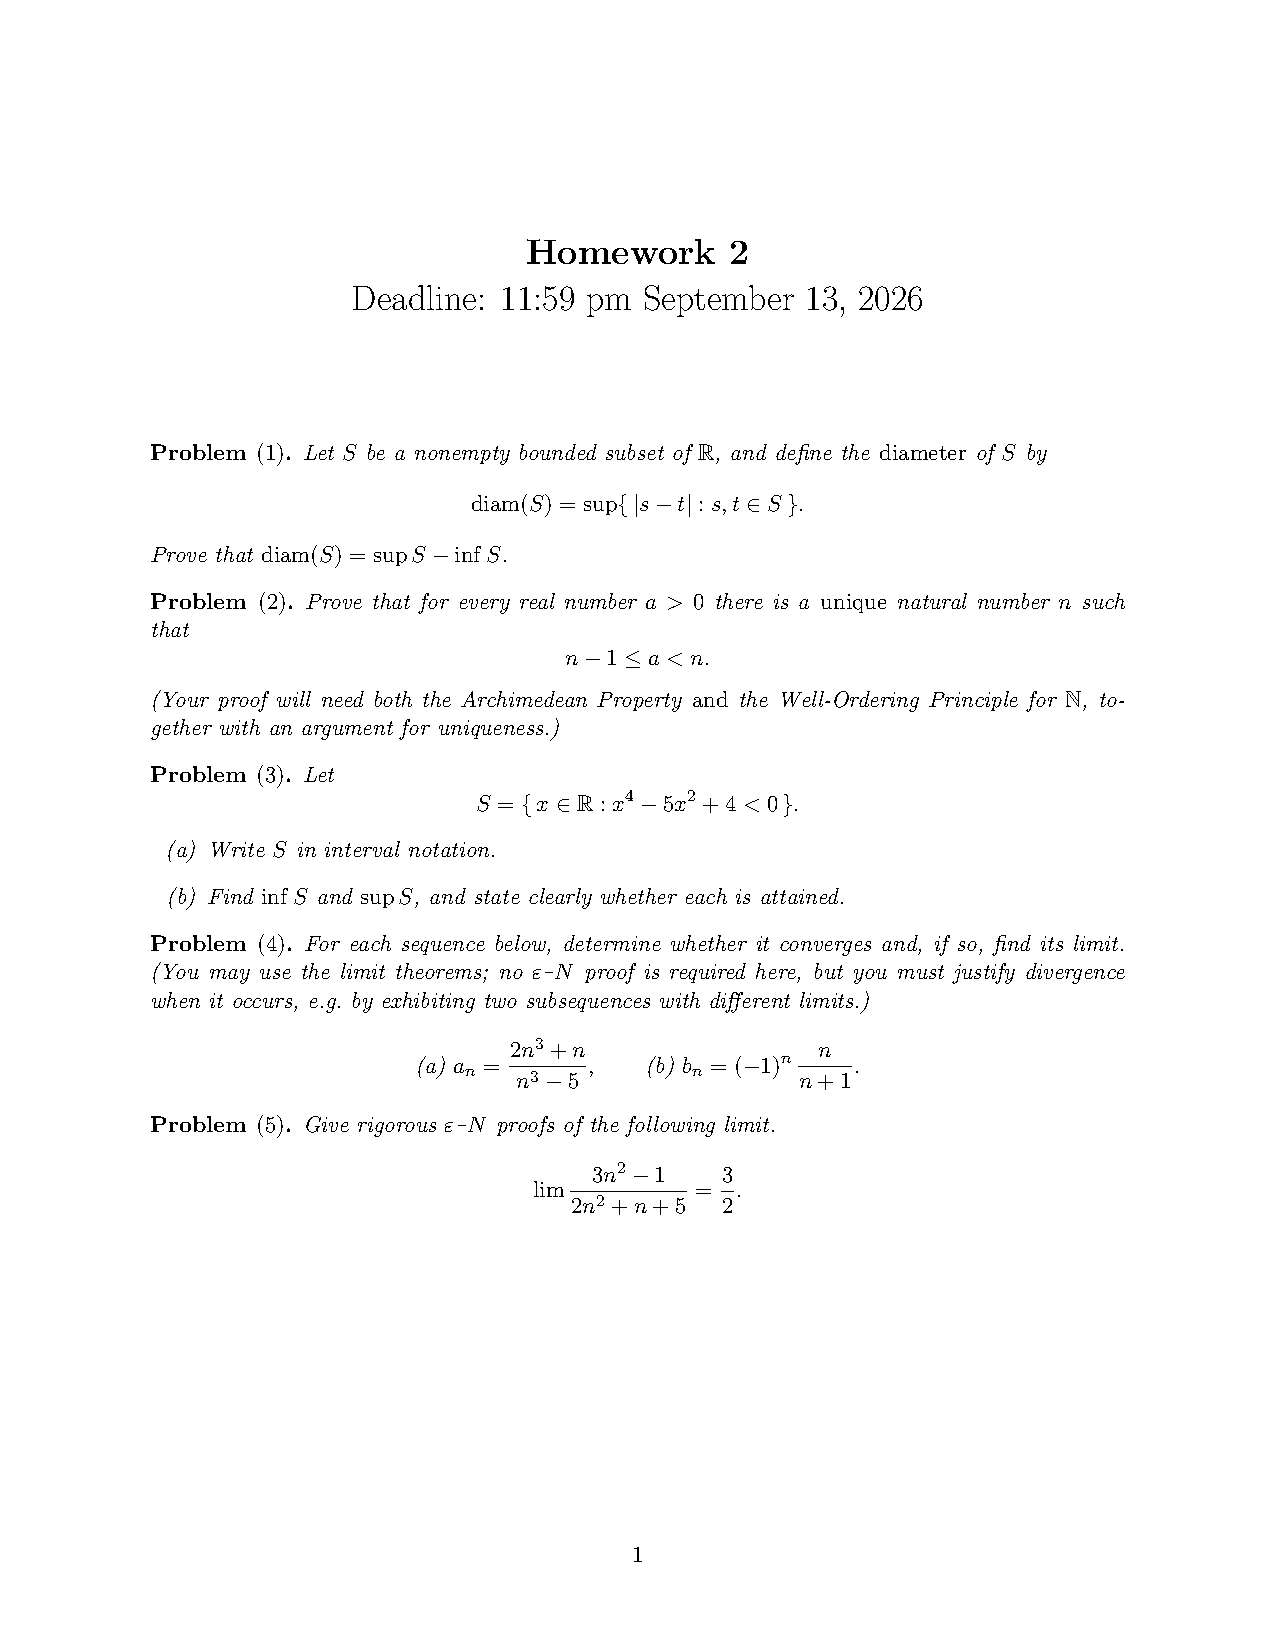
\includepdf[pages=-,pagecommand={\thispagestyle{empty}}]{hw02.pdf}
\clearpage

\section*{Solutions}
\subsubsection*{Problem 1}
\begin{solution}
    We're given a nonempty bounded subset $\mathbb{R}$, and $$\diam(S) = { \sup\{|s-t| :
    s, t \in S\}}$$
Notice that by definition of sup, $\diam(S)$ is the least upper bound of the value of
$|s-t|$ for two elements $s, t\in S$.
% \par Notice that $|s-t| = |t-s|$ for $s, t\in S$, so we can assume $s > t$ and consider the least upper bound of $s - t$.
\par We notice from the Completeness Axiom on $\mathbb{R}$ (and thus on its non empty bounded
subset), that $\sup(S)$ and $\inf(S)$ exist. 
\par We first show that $\diam(S) \le \sup(S) - \inf(S).$ \par Notice that for arbitrary $s, t$ that $\inf(S) \le s \le \sup(S)$ and $\sup(S) \ge t
\ge \inf(S)$ by definition, so subtracting these, $s - t \le \sup(S) - \inf(S)$.
\par Since s and t are defined arbitrarily, their definitions can be flipped, yielding $t - s
\le \sup(S) - \inf(S) \rightarrow |s - t| \le \sup(S) - \inf(S)$
thus $\diam(S) \le \sup(S) - \inf(S)$

Now we wish to show the other direction, namely $\diam(S) \ge \sup(S) - \inf(S)$.
\par Since $\sup(S)$ exists, $\exists s \in S \text{ such that } s + \frac{\epsilon}{2} \ge \sup(S)$
\par Considering the opposite direction, $\exists t \in S \text{ such that } t - \frac{\epsilon}{2}
\le \inf(S)$
so rearranging, we have
\begin{align}
    & s \ge \sup(S) - \frac{\epsilon}{2}\\
    & t \le \inf(S) + \frac{\epsilon}{2}\\
\end{align}
So $ s - t \ge \sup(S) - \inf(S) - \epsilon$
Flipping $t$ and $s$(where here, $$\exists t \in S \text{ s.t. } t + \frac{\epsilon}{2} \ge \sup(S), \exists s \in S \text{ s.t. } s - \frac{\epsilon}{2} \ge \inf S$$) just like above yields $$\exists s, t \in S \text{ s.t. } t - s\ge \sup(S) - \inf(S) -
\epsilon \iff |s - t| \ge \sup(S) - \inf(S) - \epsilon$$
This implies $$\diam(S) \ge \sup(S) - \inf(S) - \epsilon$$
\par So we've shown that $$\sup(S) - \inf(S) - \epsilon \le |s - t| \le \diam(S) \le \sup(S) - \inf(S)$$  so we are done, since $\diam(S)$ is bounded above by $\sup(S) - \inf(S)$ and epsilon can be arbitrarily small, bounding it below by $\sup(S) - \inf(S)$, showing equality.
% $$s \ge \sup(S) - \frac{\epsilon}{2}, t \le \inf(S) +
% \frac{\epsilon}{2}$$
% Write your proof, calculation, or argument here.
\end{solution}
\subsubsection*{Problem 2}
\begin{solution}
Given a real number $a > 0$, notice by the archimidean property, the set $$W = \{k  | k > a,
k \in \mathbb{Z}^{+}\}$$ is nonempty, and by the well ordering principle (every non
empty subset of $\mathbb{Z}^{+}$ has a unique minimum) so write $n = \min(W)$. \par Thus, for any positive real $a$, there exists $n \in \mathbb{Z}^{+} \text{ s.t } n > a$
\par \textbf{Claim $n - 1 \le a.$}
\begin{proof}
    Notice by definition, $n$ is the smallest integer in $\mathbb{Z}^{+}$ greater than
    $a$, meaning that $n - 1$ must be a or smaller, as it is not in set $W$.
\end{proof}
\textbf{Claim: n is unique}
\begin{proof}
The uniqueness can be shown by contradiction.
\par Suppose there exists $n' \in W$ such that $n' \ne \min(W)$ and $a \in [n' - 1, n')$. (so the existence of another value in W that satisfies the same condition that holds for n.)
\par Notice that $n' \ne \min(W) \rightarrow n' > \min(W)$  and since we are working on
integers, $n' \ge \min(W) + 1 \rightarrow n' - 1 \ge \min(W) > a$.
\par This yields a contradiction, as we originally had $a \in [n' - 1, n')$, yet we
showed $n' - 1 > a.$
\end{proof}
% Write your proof, calculation, or argument here.
\end{solution}
\subsubsection*{Problem 3}
\begin{solution}
    We are given the set $$S  = \{ x \in R : x^4 - 5x^2 + 4 < 0\}$$
    Notice that we can factor this expression, namely $$x^4 - 5x^2 + 4 = (x^2 - 1)(x^2 -
    4)$$
    We investigate when this is zero, and we do casework on $x^2.$
\par    \textbf{Case 1: $0 \le x^2 \le 1$}(the 0 is just from the trivial inequality) In this
    case, $x^2 - 1$ and $x^2 - 4$ are both less than or equal to 0, so the inequality is NOT
    satisfied.(either 0 or negative)
    \par \textbf{Case 2: $1 < x^2 < 4$} In this case, notice that $x^2 - 1$ is positive,
    but $x^2 - 4$ is negative, so the inequality is satisfied.
    \par \textbf{Case 3: $4 \le x^2$} In this case, notice that  $x^2 - 1$ is positive,
    and $x^2 - 4$ is greater than or equal to 0, so this expression will be greater than
    or equal to 0.

    \par Thus, the only interval that works is $1 < x^2 < 4$ works, which yields $1 < x
    < 2$ and $-1 > x > -2$
    \par So for part A, $S = \left(-2, -1\right) \cup \left(1, 2\right)$
    \par \textbf{For Part B:}
    \par $\inf(S)$ is $-2$ as every element in $S$ is greater than -2, and any element
    greater than -2 in $(-2, -1)$ can't be a lower bound, because if you consider $t \in
    (-2, -1)$, $\frac{t + (-2)}{2}$ is closer to -2 than t, a contradiction. (and if t
    is greater than or equal to -1), than any element in $(-2, -1)$ is smaller than t,
    so it can't be a lower bound.

    \par Similarly, $\sup(S)$ is $2$ because any element in $(-2, -1) \cup (1, 2)$ is
    smaller than $2$. We can do the same argument. If $t \in (1, 2)$, $\frac{t+2}{2}$ is
    closer to 2 than t, and contained in $(1, 2)$, and again if $t \in (-2, -1)$, than
    obviously any element in $(1, 2)$ is greater than t, so t can't be an upper bound.
% Write your proof, calculation, or argument here
\end{solution}
\subsubsection*{Problem 4}
\begin{solution}
   Scratch Work:
   \par we consider $|a_n - 2| < \epsilon.$ We get 
   \begin{align}
        |a_n - 2| < \epsilon
       & \frac{2n^3+n}{n^3 - 5} - \frac{2(n^3 - 5)}{n^3 - 5} < \epsilon \\
       & \frac{n+10}{n^3 - 5} < \epsilon \\
       & \frac{n+10}{n^3 - 5} > \frac{n+10}{n^3} > \frac{1}{n^2}\\ 
   \end{align}
   \noindent\textit{Claim.} For large enough n, $$\left| \frac{2n^3 + n}{n^3 -
   5} - 2\right| <\frac{2}{n^2} < \epsilon$$

\begin{proof}
    Let's cross multiply: $$\frac{n+10}{n^3 - 5} < \frac{2}{n^2}$$
    Then we get $$n^3 + 10n^2 < 2n^3 - 10 \rightarrow 10n^2 + 10 \le 11n^2 \le n^3 < 2n^3$$ which is true
    for any $n$ greater than, for example $n = 100.$ (LHS: 100,010 RHS: 2000000).
\end{proof}
Thus, we solve $\frac{2}{n^2} < \epsilon \rightarrow \frac{2}{\epsilon} < n^2$ so for
positive n, $n > \sqrt{\frac{2}{\epsilon}}$
Thus, we claim the answer holds for $$N = \max \left(100, \lceil \frac{2}{\epsilon}\rceil + 5 \right)$$,
and it holds as is shown in the scratch work.
\par \textbf{Part b) } We claim that this sequence diverges. \par This is easily shown by
considering what $a_n$ converges to when $n$ is even or odd. When $n$ is even, suppose
$n = 2k$ for $k \in \mathbb{Z}^{+}$ , we have
$$\lim_{k\rightarrow \infty}  b_{2k} = (-1)^{2k} \frac{2k}{2k + 1} = 1.$$
Yet, when considering:
 $$\lim_{k\rightarrow \infty} b_{2k+1} = (-1)^{2k + 1}\frac{2k + 1}{2k + 2} = -1$$
 Since the even and odd subsequences converge to different values, this sequence is
 divergent.
% Write your proof, calculation, or argument here.
\end{solution}
\subsubsection*{Problem 5}
\begin{solution}
    Scratch Work: Consider $\left|\frac{3n^2-1}{2n^2+n+5}-\frac{3}{2}\right| < \epsilon$
    \par Then, we can distribute to get $$\left|\frac{6n^2 - 1 - 3(2n^2 + n + 5)}{(2n^2+n+5)(2)}\right| < \epsilon$$
    which reduces to $$\frac{3n+16}{(2n^2+n+5)(2)} < \epsilon$$
    Notice that $$\frac{3n+16}{(2n^2+n+5)(2)} > \frac{3n}{(2n^2+n+5)(2)} >
    \frac{3n}{4n^2} > \frac{3}{4n}$$
    We wish to see and find a constant $c \cdot \frac{3}{4n}$ that is greater than
   $$\frac{3n+16}{(2n^2+n+5)(2)} < c\frac{3}{4n}$$
   Consider $c = 2.$
   Then, cross multiplying: $$(4n)(3n+16) < 6(2n^2+n+5)(2)$$
   So $$12n^2 + 64n < 13n^2 < 24n^2 + 12n + 60$$ 
   for $n > 64$
   Thus, we claim that $N = \max\left(65, \left\lceil \frac{3}{2\epsilon} + 5 \right\rceil\right)$
    % So we claim setting $n = \left\lceil\frac{-3}{4\epsilon} + 5\right\rceil$ will satisfy this
    % inequality.
% Write your proof, calculation, or argument here.
\end{solution}

\end{document}
